%\documentclass[12pt,draft]{IEEEtran} %!PN
\documentclass[12pt,journal,draftclsnofoot,onecolumn]{IEEEtran} 
%\documentclass[12pt]{../springer/llncs}
%\usepackage{makeidx}  % allows for indexgeneration
%\documentclass[usletter,12pt]{report}
%\documentclass[usletter,12pt]{article}
\usepackage{latexsym}
\usepackage{amssymb}
\usepackage{amsbsy}
\usepackage{amsmath}
\usepackage{multirow} 

%\usepackage{subeqnarray}
%\usepackage[subnum]{cases}
\usepackage{longtable}
\usepackage{pifont}
\usepackage{times}
%\usepackage{fancybox}
\usepackage{graphicx}
%\includegraphics*[width=xx,height=yy]{filename}
\pagestyle{plain}
%\setlength{\parskip}{0.15in}
%\setlength{\oddsidemargin}{-.0in}
%\setlength{\textwidth}{6.5in}
%\setlength{\topmargin}{-0.0in}
%\setlength{\headheight}{0.0in}
%\setlength{\headsep}{0.0in}
%\setlength{\textheight}{8.3in}
%\setlength{\textheight}{8.5in}
 
\newcommand{\rmv}[1]{}
%\renewcommand{\baselinestretch}{1.6}
%\renewcommand{\thesection}{\Roman{section}.}
%\renewcommand{\thesection}{\arabic{section}}
%\renewcommand{\thesubsection}{\Alph{subsection}.}
%\renewcommand{\thesubsection}{\arabic{section}.\arabic{subsection}.}
%\renewcommand{\theequation}{\arabic{equation}}
%%\renewcommand{\theequation}{\arabic{section}.\arabic{equation}}
%\renewcommand{\thefigure}{\arabic{figure}}
%\renewcommand{\thetable}{\arabic{table}}
%\renewcommand{\thempfootnote}{\alph{footnote}}
%\renewcommand{\thempfootnote}{\fnsymbol{footnote}}
 
\newtheorem{theorem}{Theorem}
%\newtheorem{corollary}{Corollary}
\newtheorem{algorithm}{Algorithm}
%\newtheorem{definition}{Definition}
%\newtheorem{evaluation}{Evaluation}
\newtheorem{lemma}{Lemma}
\newtheorem{example}{Example}
\newtheorem{fact}{Fact}
%\newtheorem{property}{Property}
 
%\setcounter{page}{100}
\begin{document}

%\mainmatter

\baselineskip=22 pt

\begin{titlepage}
\thispagestyle{empty}


\title{EE5414 Course Mini Project Report (BeagleBone Black)}

\author{\authorblockN{Wangchen DAI (53623708)}\\
\author{\authorblockN}{Jingwei HU (53656463)}\\
Instructor: Dr. L L CHENG\\
\authorblockA{Department  of Electronics Engineering\\
City University of Hong Kong}\\
\today}

\maketitle
\end{titlepage}


%\begin{abstract}
%
%\end{abstract}
%
%{\bf \small Key Words:}\\
%Finite field multiplication, algorithm, hardware architecture, polynomial basis.


%\newpage

%\addtocounter{\thepage}{-1}

\section{Introduction}\label{Intro}
An embedded system is a computer system with a specific function and embedded in a mechanical or electrical system. Due to the limitation of processing resurces, lower power consumption, smaller size, lower cost, and simpler operating function are the main properties of embedded computers when compared with the general ones. Embedded systems are usually based on microcontrollers or microprocessors, such as MCU, ARM, DSP and FPGA. In this project, an ARM based circuit board, BeagleBone Black (BBB), is applied as the hardware development tool. An Ubuntu14.04 terminal system, which is known as a kind of open source Linux system, is loaded into the ARM7 chip as the software development platform. Using this specified embedded system, a series of functions are developed including: LED Test, Image/Video Capture, Web Server and SQL Server Establishment. 

\section{Hardware Description and Implementation}\label{HdDes}
BBB is a low-cost, community-supported hardware platform for embedded application development. BBB board mainly contains an ARM Cortex A8 series processor, a 512MB DDR3 RAM memory, an onboard 2GB MMC chip, and some other necessary peripherals. In this project, the BBB is developed with following cables and devices: \\
$\bullet$ A MiniUSB Cable, which can be used to connect the board with PC and served as power source (limited to 500mA), network, and serial port for data transmission;\\
$\bullet$ An external DC power supply with a minimum of 1A current output;\\
$\bullet$ An USB Hub to expand the onboard USB Host port from one to four;\\
$\bullet$ An USB portable 802.11N wireless adapter;\\
$\bullet$ A Logitech HD Pro C920 Web Camera, which is a USB webcam and provides full HD 1080p video recording in wide-screen at a maximum rate of 30 frames pre second;\\
$\bullet$ A mini SD card and its corresponding USB portable card reader.\\
The detailed and connection information of all hardware cables and devices is provided in both Fig. \ref{hw1}, for block diagram view, and Fig. \ref{hw2} for real view.
\begin{figure}[ht]
	\centering
	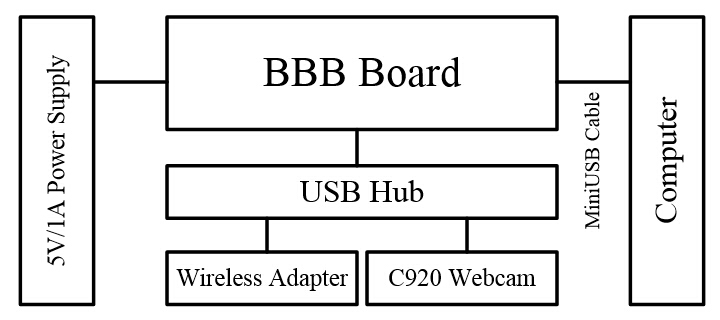
\includegraphics[width=5in]{./figs/hw1.jpg}
	\caption{Block diagram of hardware description.}
	\label{hw1}
\end{figure}
\begin{figure}[ht]
	\centering
	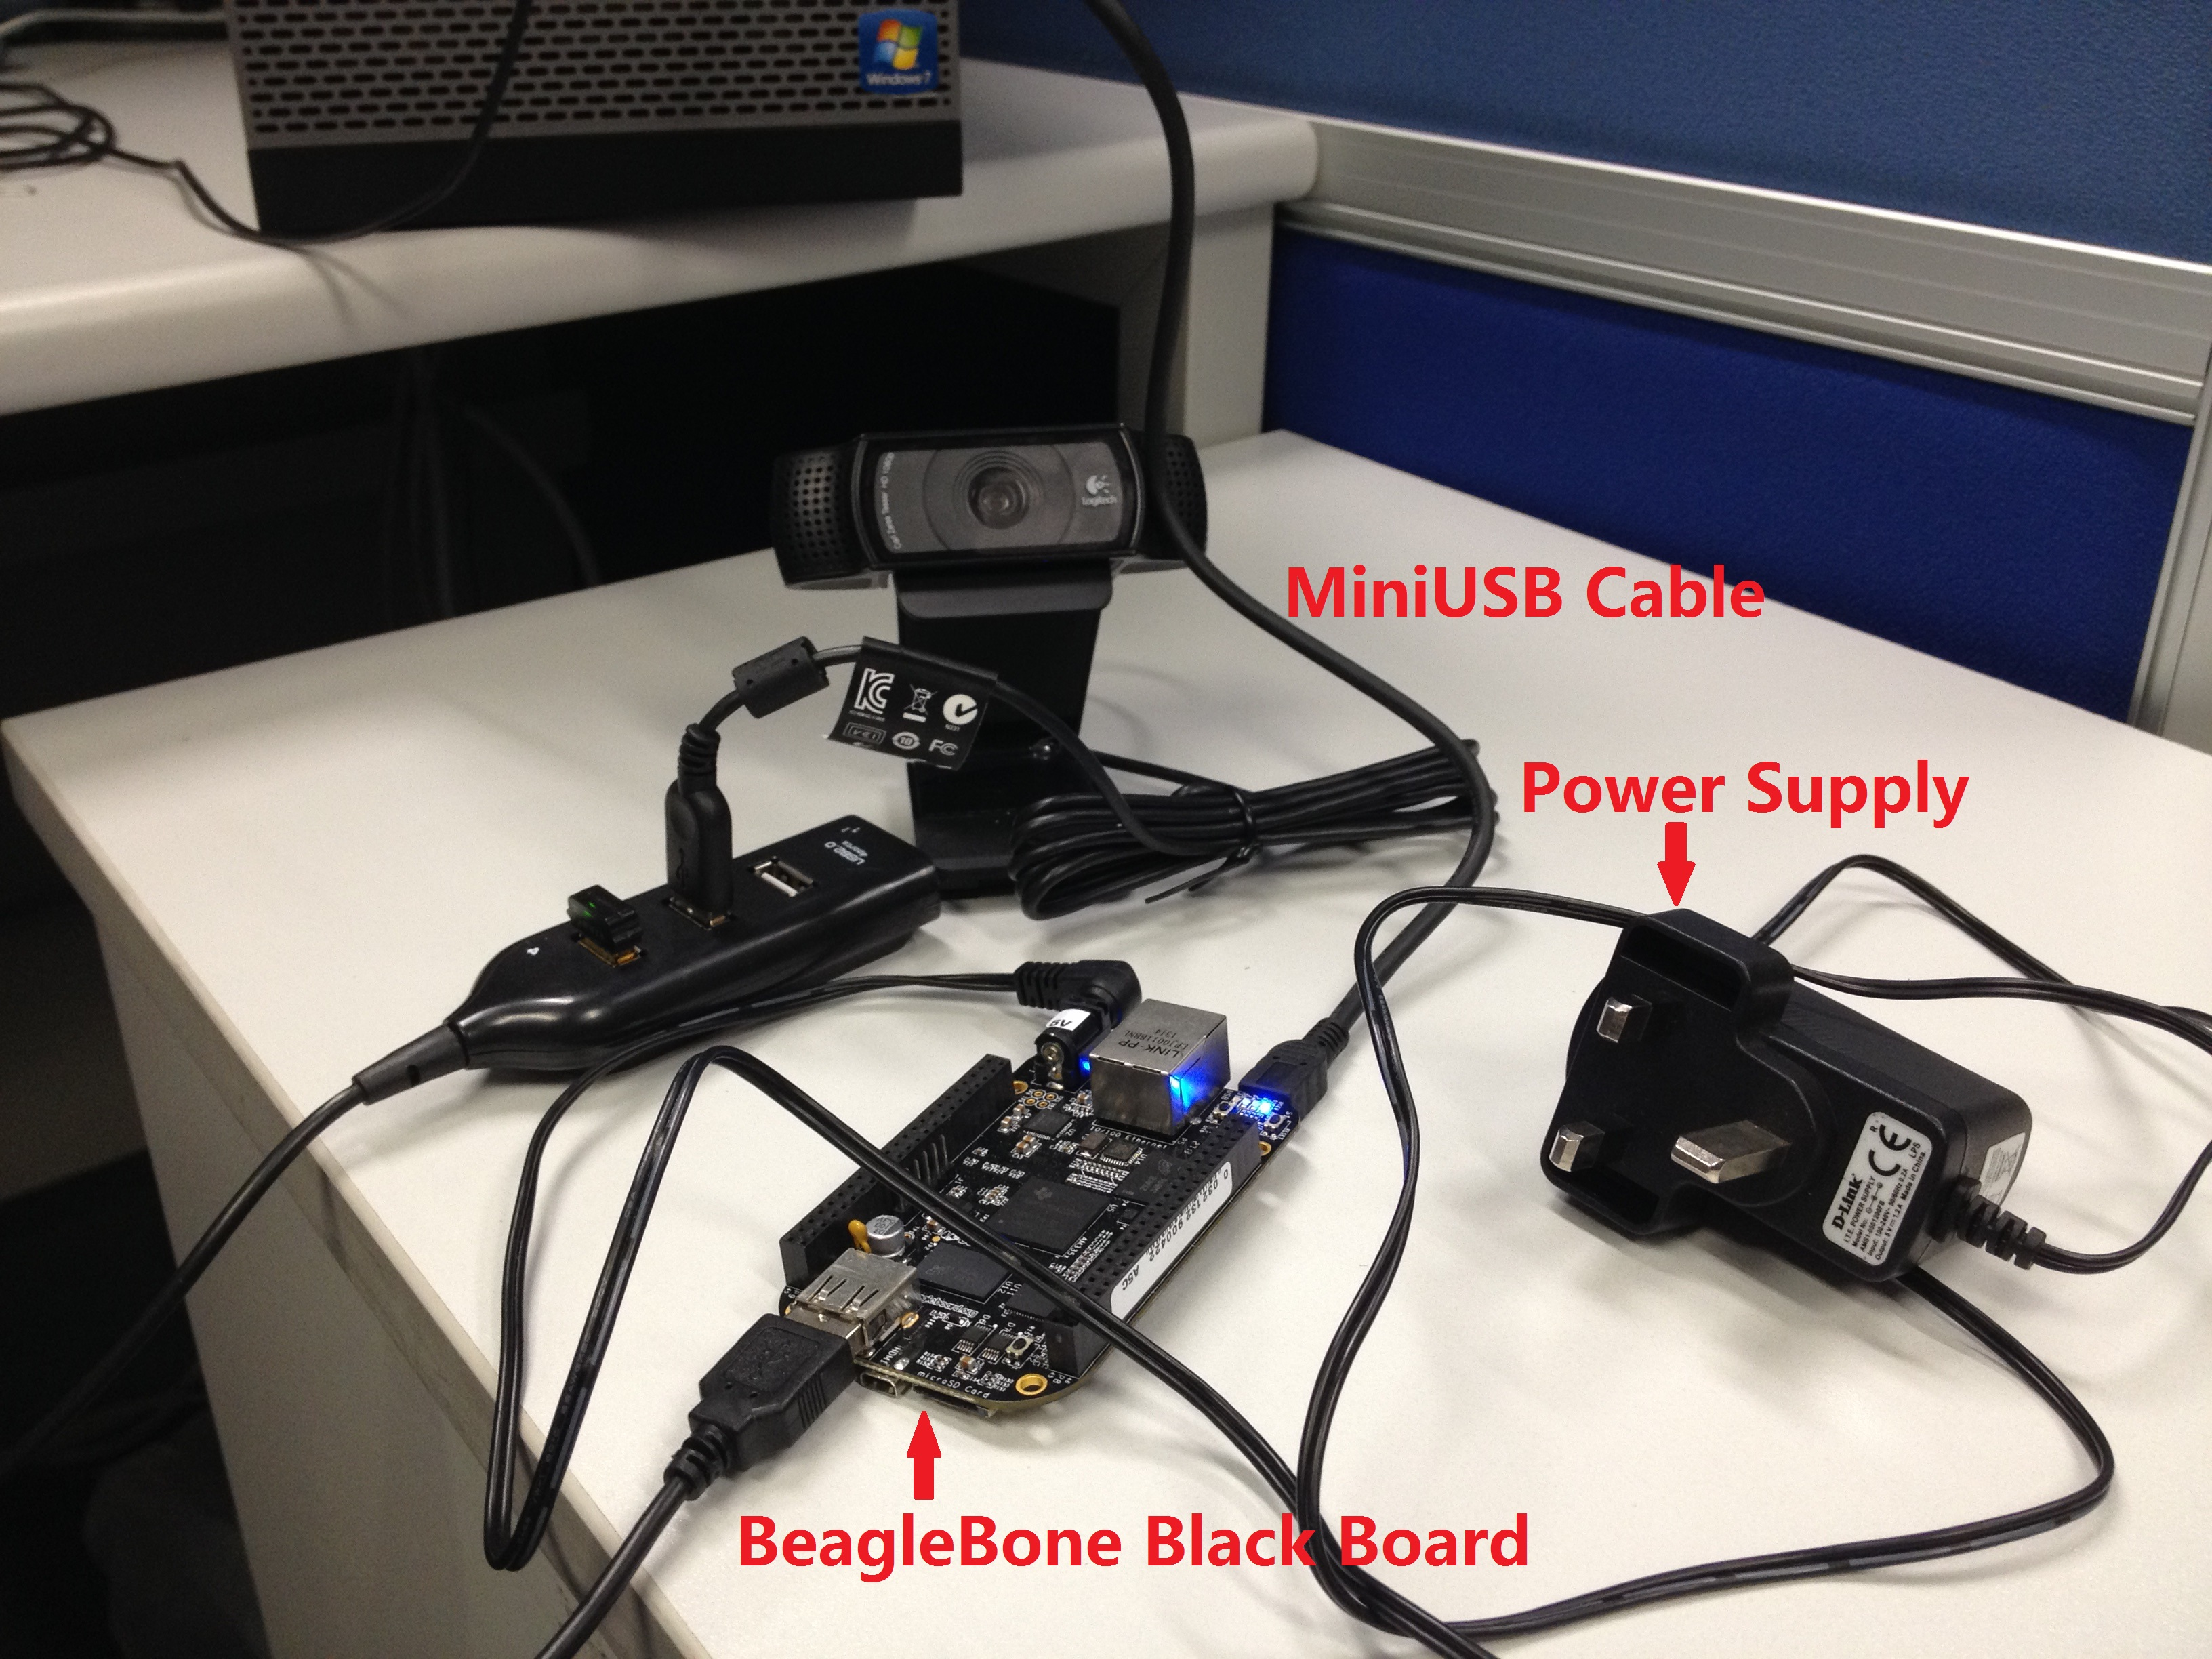
\includegraphics[width=5in]{./figs/hw2.jpg}
	\caption{Real view of hardware description.}
	\label{hw2}
\end{figure}

Both of the figures indicate the hardware setup details. First, the BBB board is connected to a PC using the MiniUSB Cable. Via the cable, the BBB board could not only receives a 5V/500mA power supply provided by PC's USB port, but also accesses to the Internet by setting up Windows ICS, in addition, users could operate Linux instructions through specific Windows-based software clients. Second, in case of unexpected system shutdown issue caused by current exceeding (current supply using MiniUSB Cable is set at a maximum of 500mA), an external power supply is used. Third, an USB Hub is connected to the onboard host USB port for expanding the port from one to four. Finally, the Logitech C920 webcam is connected to the USB Hub with its attached USB cable, together with a USB portable wireless adapter. Note that in this project, the BBB board could have an alternative way to access the Internet: getting access to a Wifi or a Hotspot connection via the wireless adapter; and the system could have two different IP address for Ethernet and wireless connection, respectively.






\section*{Acknowledgment}
This work was supported with an NSERC Discovery Grant.

\begin{thebibliography}{1} 
\item
\end{thebibliography}
%\bibliographystyle{latex8} \bibliography{latex8}

\end{document}



%\bibliographystyle{plain}
%\bibliography{source}

